% =============================================================================
% File      : ex_doc_2-10.tex -- example 2.10
% Author    : Jürgen Hackl <hackl.j@gmx.at>
% Creation  : 2019-08-14
% Time-stamp: <Wed 2019-08-14 16:52 juergen>
%
% Copyright (c) 2019 Jürgen Hackl <hackl.j@gmx.at>
% =============================================================================
\documentclass{standalone}
\usepackage{../../tikz-network}
\begin{document}
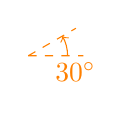
\begin{tikzpicture}
  \Vertex[label=A,position=below]{A}
  \Vertex[x=1,label=B,position=below,distance=2mm]{B}
  \Vertex[x=2,label=C,position=30,distance=1mm]{C}
  \draw[orange,dashed](2,0) --++ (7mm,0mm)(2,0)--++(30:7mm);
  \draw[orange,->] (2.5,0) arc (0:30:5mm);
  \node[orange] (x) at (2.6,-.2) {$30^\circ$};
\end{tikzpicture}
\end{document}
% =============================================================================
% eof

%%% Local Variables:
%%% mode: latex
%%% TeX-master: t
%%% End:
